\documentclass{article}
\usepackage[margin=0.3in]{geometry}
\usepackage{graphicx}
\usepackage{caption}
\usepackage{color}
\usepackage{subcaption}
\usepackage{hyperref}
\graphicspath{ {/asay/Desktop/images/} }
\usepackage{xepersian}


\title{پاسخ تمرین تئوری دوم درس هوش مصنوعی}

\author{امیر حسین عاصم یوسفی \\ ۹۶۱۱۰۳۲۳}
\settextfont{B Nazanin}

\begin{document}
	\maketitle
	\section*{مسئله ۱ }
	\subsection*{۱}
	تابع هزینه یا تابع ضرر در واقع میزان خطای الگوریتم در هر بار اجرا شدن است که برابراست با مجموع فاصله هر داده تا مقدار واقعی آن که به صورت زیر می باشد  :
	\begin{center}
		\lr{Cost Function = $\sum  _t ||w_t - w^\prime _t||^2$}
	\end{center}
بناربراین مقدار بالا باید مینیمم شود  . 
\subsection*{۲}
فرض می کنیم داده 
\lr{$X_i$}
در دسته منفی ها قرار می گرفته بنابراین در صورتی اشتباه دسته بندی می شود که 
\lr{$X_i  \ . \ W_t >0$}
باشد بنابر الگوریتم وزن مرحله بعد به صورت زیر میشود :
\begin{center}
	$W_{t+1} = W_t - X_i \Rightarrow X_i \ . \ W_{t+1} = W_t \ . \ X_i  - X_i \ . \ X_i = W_t X_i - |X_i|^2$
\end{center}

بنابراین مقدار 
\lr{$X_i \ .\ W_{t+1}$}
برابر است با 
\lr{$W_t \ . \ X_i$}
که یک مقدار مثبت از آن کم شده است بنابراین قبلا مثبت بوده و الان به سمت منفی ها حرکت می کند بنابراین در جهت بهبود دسته بندی 
\lr{$X_i$}
تغییر می کند . \\
حال فرض می کنیم داده 
\lr{$X_i$}
جزو دسته مثبت ها قرار می گرفته درصورتی اشتباه در دسته بندی صورت می گیرد که 
\lr{$X_i  \ . \ W_t <0$}
بنابر الگوریتم ، وزن در مرحله بعدی به صورت زیر تغییر می کند  :‌
\begin{center}
	$W_{t+1} = W_t + X_i \Rightarrow X_i \ . \ W_{t+1} = W_t \ . \ X_i  + X_i \ . \ X_i = W_t X_i + |X_i|^2$
\end{center}
بنابراین مقدار 
\lr{$X_i \ .\ W_{t+1}$}
برابر است با 
\lr{$W_t \ . \ X_i$}
که با یک مقدار مثبت جمع  شده است بنابراین قبلا منفی بوده و الان به سمت مثبت ها حرکت می کند بنابراین در جهت بهبود دسته بندی 
\lr{$X_i$}
تغییر می کند .



\hrule


\section*{مسئله ۳}
ابتدا برای هر دو کلاس 
\lr{A}
و 
\lr{B}
یک وزن تعیین می کنیم 
\begin{flushleft}
	\begin{enumerate}
		\item \lr{$W_A$ = (bias = 1 , f1 =0 , f2 =0 , f3 = 0)}
		\item \lr{$W_B = $ (bias = 0 , f1= 0 , f2 =0 , f3 = 0)}
	\end{enumerate}
\end{flushleft}
حال داده ها را به ترتیب از چپ به راست به الگوریتم میدهیم(مقدار
\lr{bias}
برای تمام داده ها برابر با یک می باشد  . 
)
 و الگوریتم پرسپترون را اجرا می کنیم تا جایی که بردار وزن هر کلاس
ثابت باقی بماند  : 
\subsection*{\lr{First Iteration}}
داده 
\lr{D1}
به الگوریتم داده می شود  داریم  : 
\lr{$W_{D1} = $ (bias = 1 ,f1 =  2 ,f2 =  1,f3 =  0.5)}
\begin{center}
	\lr{$W_A  \ .  \ W_{D1} $ = 1}
	\\
	\lr{$W_B \ . \ W_{D1}$ = 0}
\end{center}
بنابراین با توجه به مقادیر بالا داده 
\lr{D1}
در کلاس 
\lr{A}
قرار می گیرد که درست است بنابراین بردار وزن هر دو کلاس بدون تغییر باقی می ماند  . 
\\
حال داده دوم را به الگوریتم میدهیم  
\lr{$W_{D2} = $(1 , 10 , 2 , 5)}
 : 
 \begin{center}
 	\lr{$W_A  \ . \ W_{D2}$ = 1}
 	\\
 	\lr{$W_B \ . \ W_{D2}$ = 0}
 \end{center}
بنابراین با توجه به مقادیر بالا داده دوم در کلاس 
\lr{A}
قرار می گیرد که اشتباه است بنابراین وزن ها را به روز می کنیم 
\begin{center}
	\lr{$W_A(New)$ = $W_A  \ - \ W_{D2}$ = (1 , 0 , 0 , 0) - (1 , 10 , 2 , 5) = (0 , -10 , -2 , -5)}
	\\
	\lr{$W_B (New) = $$W_B \ + \ W_{D2}  = $(0 ,0,0,0) + (1 , 10 ,2 ,5) = (1 , 10 ,2 ,5)}
\end{center}
حال با وزن های جدید بالا داده سوم را به الگوریتم می دهیم  
\lr{$W_{D3} = $(1 , 10 , 7 , 0.1)}
:
\begin{center}
		\lr{$W_A(New)  \ .  \ W_{D3} $ = -114.5}
	\\
	\lr{$W_B(New) \ . \ W_{D3}$ = 115.5}
\end{center}
  بنابراین با توجه به مقادیر بالا داده سوم در کلاس 
  \lr{B}
  قرار می گیرد که درست است ، پس مقادیر وزن ها تغییری نمی کند  . \\
  حال داده چهارم را وارد می کنیم 
  \lr{$W_{D4} = $(1 , 3, 3, 9)}
  بنابراین 
  \begin{center}
  		\lr{$W_A(New)  \ .  \ W_{D4} $ = -81}
  	\\
  	\lr{$W_B(New) \ . \ W_{D4}$ = 82}
  \end{center}
با توجه به مقادیر بالا می توان دید که داده چهارم در کلاس 
\lr{B}
قرار می گیرد که اشتباه است بنابراین وزن ها را به روز می کنیم  : 
\begin{center}
	\lr{$W_A(New2) =  W_A(New) \ + \ W_{D4}$ = (0 , -10 , -2 , -5) + (1 , 3, 3, 9) = (1 , -7 , 1 , 4)}
	\\
	\lr{$W_B(New2) = W_B(New ) \ - \ W_{D4} = $(1 , 10 , 2 , 5) - (1 , 3 ,3 ,9) = (0 , 7 , -1 , -4)}
\end{center}
حال داده پنجم را وارد می کنیم  
\lr{$W_{D5} = $(1 ,2 , 9 ,8)}
:
\begin{center}
		\lr{$W_A(New2)  \ .  \ W_{D5} $ = 28}
	\\
	\lr{$W_B(New2) \ . \ W_{D5}$ = -27}
\end{center}
بنابراین طبق مقادیر بالا داده پنجم در کلاس 
\lr{A}
قرار می گیرد که درست است بنابراین مقادیر وزن ها ثابت می ماند  . \\
\subsection*{\lr{Second Iteration}}
با مقدار وزن های زیر به دوباره داده ها رابررسی میکنیم : 
\begin{center}
	\lr{$W_A$ = (1 , -7 , 1 , 4)}
	\\
	\lr{$W_B$ = (0 , 7 , -1 , -4)}
\end{center}
داده اول را وارد می کنیم 
\begin{center}
		\lr{$W_A  \ .  \ W_{D1} $ = -10}
	\\
	\lr{$W_B \ . \ W_{D1}$ = 12}
\end{center}
با توجه به مقادیر داده اول داخل کلاس 
\lr{B}
قرار می گیرد که اشتباه است بنابراین باید مقدار وزن ها را تغییر دهیم   : 
\begin{center}
		\lr{$W_A(New)$ = $W_A  \ + \ W_{D1}$ = (1 , -7 , 1 , 4) + (1 , 2 , 1 , 0.5) = (2 , -5 , 2 , 4.5)}
	\\
	\lr{$W_B (New) = $$W_B \ - \ W_{D1}  = $(0 ,7,-1,-4) - (1 , 2 ,1, 0.5) = (-1 , 5 ,-2 ,-4.5)}
\end{center}
حال داده دوم را وارد می کنیم :
\begin{center}
		\lr{$W_A(New)  \ .  \ W_{D2} $ =-21.5}
	\\
	\lr{$W_B(New) \ . \ W_{D2}$ =22.5 }
\end{center}
با توجه به مقادیر می بینیم که داده دوم در کلاس 
\lr{B}
قرار می گیرد که درست است بنابراین مقادیر وزن ها ثابت می ماند  . \\
حال داده سوم را وارد می کنیم  : 
\begin{center}
		\lr{$W_A(New)  \ .  \ W_{D3} $ = -33.55}
	\\
	\lr{$W_B(New) \ . \ W_{D3}$ = 34.55}
\end{center}
با توجه به مقادیر بالا می توان دید که داده سوم به کلاس 
\lr{B}
تعلق می گیرد که درست است .بنابراین مقادیر وزن ها ثابت می ماند  . \\
حال  داده چهارم را وارد می کنیم  : 
\begin{center}
		\lr{$W_A(New)  \ .  \ W_{D4} $ =33.5}
	\\
	\lr{$W_B(New) \ . \ W_{D4}$ = -32.5}
\end{center}
که با توجه به مقادیر بالا می توان دید که داده چهارم در کلاس 
\lr{A}
قرار می گیرد که درست است . بنابراین مقادیر وزن ها ثابت می ماند  . \\
حال داده پنجم را وارد می کنیم  : 
\begin{center}
		\lr{$W_A(New)  \ .  \ W_{D5} $ =46 }
	\\
	\lr{$W_B(New) \ . \ W_{D5}$ = -45}
\end{center}
با توجه به مقادیر بالا می توان دید که داده پنجم در کلاس 
\lr{A}
قرار می گیرد بنابراین مقادیر وزن ها ثابت می ماند  . 
\subsection*{\lr{Third Iteration}}
از مرحله قبل مقادیر وزن ها به صورت زیر است  :‌
\begin{center}
		\lr{$W_A  $ = (2 , -5 , 2 , 4.5)}
	\\
	\lr{$W_B$ = (-1 , 5 , -2 , -4.5)}
\end{center}
حال داده اول را وارد می کنیم   : 
\begin{center}
		\lr{$W_A \ .  \ W_{D1} $ = -3.75}
	\\
	\lr{$W_B \ . \ W_{D1}$ = 4.75 }
\end{center}
با توجه به مقادیر بالا داده اول در کلاس 
\lr{B}
قرار می گیرد که اشتباه است بنابراین باید وزن ها را 
\lr{update}
کنیم  : 
\begin{center}
		\lr{$W_A(New)$ = $W_A  \ + \ W_{D1}$ = (2 , -5 , 2 , 4.5) + (1 , 2 , 1 , 0.5) = (3 , -3 , 3 , 5)}
	\\
	\lr{$W_B (New) = $$W_B \ - \ W_{D1}  = $(-1 ,5,-2,-4.5) - (1 , 2 ,1, 0.5) = (-2 , 3 ,-3 ,-5)}
\end{center}
حال داده دوم را وارد می کنیم  : 
\begin{center}
		\lr{$W_A(New)  \ .  \ W_{D2} $ =4 }
	\\
	\lr{$W_B(New) \ . \ W_{D2}$ = -3}
\end{center}
که با توجه به مقادیر بالا داده دوم در کلاس 
\lr{A}
قرار می گیرد که اشتباه است بنابراین وزن ها را باید 
\lr{update}
کنیم  :‌
\begin{center}
		\lr{$W_A(New2) =  W_A(New) \ - \ W_{D2}$ = (3 , -3 , 3 , 5) - (1 , 10, 2, 5) = (2 , -13 , 1 , 0)}
	\\
	\lr{$W_B(New2) = W_B(New ) \ + \ W_{D2} = $(-2 , 3 , -3 , -5) + (1 , 10 ,2 ,5) = (-1 , 13 , -1 , 0)}
\end{center}
حال داده سوم را وارد می کنیم :
\begin{center}
		\lr{$W_A(New2)  \ .  \ W_{D3} $ =-124 }
	\\
	\lr{$W_B(New2) \ . \ W_{D3}$ = 122}
\end{center}
با توجه به مقادیر بالا داده سوم در کلاس 
\lr{B}
قرار میگیرد که درست است پس مقادیر وزن ها را تغییر نمی دهیم  . \\
داده چهارم را وارد می کنیم  : 
\begin{center}
		\lr{$W_A(New2)  \ .  \ W_{D4} $ =-34 }
	\\
	\lr{$W_B(New2) \ . \ W_{D4}$ = 35}
\end{center}
با توجه به محاسبات بالا داده چهارم در کلاس 
\lr{B}
قرار می گیرد که اشتباه است بنابراین باید وزن ها را 
\lr{update}
کنیم  : 
\begin{center}
		\lr{$W_A(New3) =  W_A(New2) \ - \ W_{D4}$ = (2 , -13 , 1 , 0) - (1 , 3, 3, 9) = (1 , -16 , 0 , -9)}
	\\
	\lr{$W_B(New3) = W_B(New2) \ + \ W_{D4} = $(-1 , 13 , -1 , 0) + (1 , 3 ,3 ,9) = (0 , 16 , 2 , 0)}
\end{center}
حال داده پنجم را وارد می کنیم  : 
\begin{center}
		\lr{$W_A(New3)  \ .  \ W_{D5} $ =-103}
	\\
	\lr{$W_B(New3) \ . \ W_{D5}$ = 50}
\end{center}
بنابراین داده پنجم در کلاس 
\lr{B}
قرار می گیرد که اشتباه است بنابراین باید وزن ها را 
\lr{update}
کنیم  : 
\begin{center}
		\lr{$W_A(New4) =  W_A(New3) \ - \ W_{D5}$ = (1 , -16 , 0 , -9) - (1 , 2, 9, 8) = (0 , -18 , -9 , -17)}
	\\
	\lr{$W_B(New4) = W_B(New3) \ + \ W_{D5} = $(0 , 16 , 2 , 0) + (1 , 2 ,9 ,8) = (1 , 18 , 4 , 0)}
\end{center}
بعد از مرحله سوم می بینیم که در این مرحله ۴ بار بردار وزن را به روز رسانی کردیم و فقط دو داده را درست تشخیص دادیم  
ولی در 
\lr{Second Iteration}
دیدم که با یک بار به روز کردن وزن ها توانستیم ۴ داده را درست تشخیص دهیم بنابراین دقت در مرحله دوم برابر با ۸۰ درصد می باشد این  در حالی است که در مرحله سوم ۴۰ درصد می باشد بنابراین اگر اجرای الگوریتم را ادامه دهیم بردار های وزن 
\lr{overfit}
می شوند بنابراین بهترین مقدار برای بردارهای وزن دو کلاس 
\lr{A}
و
\lr{B}
برابر است با 
\begin{center}
	\lr{$W_A  $ = (2 , -5 , 2 , 4.5)}
\\
\lr{$W_B$ = (-1 , 5 , -2 , -4.5)}
\end{center}
\hrule
\section*{مسئله ۴}
\subsection*{هوشنگ حداکثر ۲ خواهر دارد  } : 
\begin{center}
	$\forall x , y , z ((HasSibling(hosing , x) \land Female(y) \land HasSibling (hoshang , y) \land Female(y) \land HasSibling(hoshang , z ) \land Female(z)) \Rightarrow (x=y \lor y=z \lor y=z)) $
\end{center}
\subsection*{همه دانشجویان حداقل یک درس را برداشته اند}
به ازای هر دانشجو یک درس وجود دارد که آن دانشجو آن را گرفته است 
\begin{center}
	$\forall x \exists y(Taken(x,y))$
\end{center}
که 
\lr{x}
بیانگر دانشجو و 
\lr{y}
بیانگر درس می باشد 
\subsection*{هیچ دانشجویی نمی تواند تمام دانشجویان را گول بزند }
یعنی به ازای هر دانشجو یک دانشجو وجود دارد که از آن دانشجو گول نمی خورد 
\begin{center}
	$ \forall x\exists y(Student(x) \land Student(y) \Rightarrow \neg Deceive(x,y))$
\end{center}
\subsection*{تنها یک دانشجو درس هوش را افتاده است }
\begin{center}
	$ \exists x(Fail(x,AI) \land \forall y : (Fail(y , AI) \Rightarrow x = y))$
\end{center}
\hrule
\section*{مسئله۵}
\subsection*{همسایگان خوب حیوانات پر سروصدا ندارند }
\begin{center}
	$ \forall x\forall y(GoodNeighbour(x) \land HaveAnimal(x,y) \Rightarrow \neg Noisy(y))$
\end{center}
\subsection*{اگرکسی گربه داشته باشد آنگاه موش ندارد }
\begin{center}
	$ \forall x\forall y(HaveAnimal(x,y) \land IsCat(y) \Rightarrow \neg HaveMouse(x))$
\end{center}
\subsection*{همه سگ ها حیوانات پر سر و صدایی هستند}
\begin{center}
	$ \forall y (IsDog(y) \Rightarrow Noisy(y))$
\end{center}
\subsection*{علی سگ یا گربه دارد }
\begin{center}
	$ \forall y(HaveAnimal(Ali,y)\Rightarrow (IsDog(y) \lor IsCat(y)))$
\end{center}
\subsection*{حکم : اگر علی همسایه خوبی باشد ، آنگاه موش ندارد }
\begin{center}
	$ \forall y (GoodNeighbour(Ali)  \land HaveAnimal(Ali,y)\Rightarrow \neg HaveMouse(Ali))$
\end{center}
حال جملات را به صورت 
\lr{CNF}
می نویسیم  : 
\begin{center}
	\begin{enumerate}
		\item $ \neg GoodNeighbour(x) \lor\neg HaveAnimal(x,y)  \lor  \neg Noisy(y)$
		\item $ \neg HaveAnimal(x,y) \lor \neg IsCat(y)\lor \neg HaveMouse(x)$
		\item $ \neg IsDog(y) \lor Noisy(y)$
		\item $ \neg HaveAnimal(Ali,y) \lor IsDog(y) \lor IsCat(y)$
		\item \textbf{$ \neg GoodNeighbour(Ali) \lor \neg HaveAnimal(Ali,y) \lor \neg HaveMouse(Ali)$}
	\end{enumerate}
\end{center}
حال 
\lr{NOT}
عبارت پنجم(حکم)  را به 
\lr{KB}
اضافه می کنیم بنابراین 
\lr{KB}
به صورت زیر است  : 
\begin{center}
	\begin{enumerate}
		\item $ \neg GoodNeighbour(x) \lor\neg HaveAnimal(x,y)  \lor \neg Noisy(y)$
		\item $ \neg HaveAnimal(x,y) \lor \neg IsCat(y)\lor \neg HaveMouse(x)$
		\item $ \neg IsDog(y) \lor Noisy(y)$
		\item $ \neg HaveAnimal(Ali,y) \lor IsDog(y) \lor IsCat(y)$
		\item $ GoodNeighbour(Ali)$
		\item $HaveMouse(Ali)$
		\item $HaveAnimal(Ali,y)$
	\end{enumerate}
\end{center}
ابتدا عبارات ۱ و ۵ را به ازای 
\lr{x = Ali}
با یک دیگر 
\lr{resolve}
می کنیم بنابراین 
\lr{KB}
به شکل زیر است  : 
\begin{center}
	\begin{enumerate}
		\item $ \neg GoodNeighbour(x) \lor\neg HaveAnimal(x,y)  \lor \neg Noisy(y)$
		\item $ \neg HaveAnimal(x,y) \lor \neg IsCat(y)\lor \neg HaveMouse(x)$
		\item $ \neg IsDog(y) \lor Noisy(y)$
		\item $ \neg HaveAnimal(Ali,y) \lor IsDog(y) \lor IsCat(y)$
		\item $ GoodNeighbour(Ali)$
		\item $HaveMouse(Ali)$
		\item $HaveAnimal(Ali,y)$
		\item $\neg HaveAnimal(Ali,y) \lor \neg Noisy(y)$
	\end{enumerate}
\end{center}
حال دو عبارت ۷ و۸ را با یک دیگر 
\lr{resolve}
می کنیم بنابراین 
\lr{KB}
به شکل زیر می باشد  : 
\begin{center}
	\begin{enumerate}
		\item $ \neg GoodNeighbour(x) \lor\neg HaveAnimal(x,y)  \lor \neg Noisy(y)$
		\item $ \neg HaveAnimal(x,y) \lor \neg IsCat(y)\lor \neg HaveMouse(x)$
		\item $ \neg IsDog(y) \lor Noisy(y)$
		\item $ \neg HaveAnimal(Ali,y) \lor IsDog(y) \lor IsCat(y)$
		\item $ GoodNeighbour(Ali)$
		\item $HaveMouse(Ali)$
		\item $HaveAnimal(Ali,y)$
		\item $\neg HaveAnimal(Ali,y) \lor \neg Noisy(y)$
		\item $ \neg Noisy(y)$
	\end{enumerate}
\end{center}
حال دو عبارت ۹ و۳ را با یکدیگر 
\lr{resolve}
می کنیم پس  :
\begin{center}
	\begin{enumerate}
		\item $ \neg GoodNeighbour(x) \lor\neg HaveAnimal(x,y)  \lor \neg Noisy(y)$
		\item $ \neg HaveAnimal(x,y) \lor \neg IsCat(y)\lor \neg HaveMouse(x)$
		\item $ \neg IsDog(y) \lor Noisy(y)$
		\item $ \neg HaveAnimal(Ali,y) \lor IsDog(y) \lor IsCat(y)$
		\item $ GoodNeighbour(Ali)$
		\item $HaveMouse(Ali)$
		\item $HaveAnimal(Ali,y)$
		\item $\neg HaveAnimal(Ali,y) \lor \neg Noisy(y)$
		\item $ \neg Noisy(y)$
		\item $\neg IsDog(y)$
	\end{enumerate}
\end{center}
حال دو عبارت ۲ و۶ را به ازای 
\lr{X = Ali}
با یک دیگر 
\lr{resolve}
می کنیم پس  : 
\begin{center}
	\begin{enumerate}
		\item $ \neg GoodNeighbour(x) \lor\neg HaveAnimal(x,y)  \lor \neg Noisy(y)$
		\item $ \neg HaveAnimal(x,y) \lor \neg IsCat(y)\lor \neg HaveMouse(x)$
		\item $ \neg IsDog(y) \lor Noisy(y)$
		\item $ \neg HaveAnimal(Ali,y) \lor IsDog(y) \lor IsCat(y)$
		\item $ GoodNeighbour(Ali)$
		\item $HaveMouse(Ali)$
		\item $HaveAnimal(Ali,y)$
		\item $\neg HaveAnimal(Ali,y) \lor \neg Noisy(y)$
		\item $ \neg Noisy(y)$
		\item $\neg IsDog(y)$
		\item $\neg HaveAnimal(Ali,y) \lor \neg IsCat(y)$
	\end{enumerate}
\end{center}
حال دو عبارت ۱۱ و ۷ را با یکدیگر 
\lr{resolve}
می کنیم پس : 
\begin{center}
	\begin{enumerate}
		\item $ \neg GoodNeighbour(x) \lor\neg HaveAnimal(x,y)  \lor \neg Noisy(y)$
		\item $ \neg HaveAnimal(x,y) \lor \neg IsCat(y)\lor \neg HaveMouse(x)$
		\item $ \neg IsDog(y) \lor Noisy(y)$
		\item $ \neg HaveAnimal(Ali,y) \lor IsDog(y) \lor IsCat(y)$
		\item $ GoodNeighbour(Ali)$
		\item $HaveMouse(Ali)$
		\item $HaveAnimal(Ali,y)$
		\item $\neg HaveAnimal(Ali,y) \lor \neg Noisy(y)$
		\item $ \neg Noisy(y)$
		\item $\neg IsDog(y)$
		\item $\neg HaveAnimal(Ali,y) \lor \neg IsCat(y)$
		\item $\neg IsCat(y)$
	\end{enumerate}
\end{center}
حال دو عبارت ۴ و ۷ را با یکدیگر 
\lr{Resolve}
می کنیم پس : 
\begin{center}
	\begin{enumerate}
		\item $ \neg GoodNeighbour(x) \lor\neg HaveAnimal(x,y)  \lor \neg Noisy(y)$
		\item $ \neg HaveAnimal(x,y) \lor \neg IsCat(y)\lor \neg HaveMouse(x)$
		\item $ \neg IsDog(y) \lor Noisy(y)$
		\item $ \neg HaveAnimal(Ali,y) \lor IsDog(y) \lor IsCat(y)$
		\item $ GoodNeighbour(Ali)$
		\item $HaveMouse(Ali)$
		\item $HaveAnimal(Ali,y)$
		\item $\neg HaveAnimal(Ali,y) \lor \neg Noisy(y)$
		\item $ \neg Noisy(y)$
		\item $\neg IsDog(y)$
		\item $\neg HaveAnimal(Ali,y) \lor \neg IsCat(y)$
		\item $\neg IsCat(y)$
		\item $IsDog(y) \lor IsCat(y)$
	\end{enumerate}
\end{center}
حال دو عبارت ۱۳ و۱۲ را با یکدیگر 
\lr{resolve}
می کنیم پس  :
\begin{center}
	\begin{enumerate}
		\item $ \neg GoodNeighbour(x) \lor\neg HaveAnimal(x,y)  \lor \neg Noisy(y)$
		\item $ \neg HaveAnimal(x,y) \lor \neg IsCat(y)\lor \neg HaveMouse(x)$
		\item $ \neg IsDog(y) \lor Noisy(y)$
		\item $ \neg HaveAnimal(Ali,y) \lor IsDog(y) \lor IsCat(y)$
		\item $ GoodNeighbour(Ali)$
		\item $HaveMouse(Ali)$
		\item $HaveAnimal(Ali,y)$
		\item $\neg HaveAnimal(Ali,y) \lor \neg Noisy(y)$
		\item $ \neg Noisy(y)$
		\item $\neg IsDog(y)$
		\item $\neg HaveAnimal(Ali,y) \lor \neg IsCat(y)$
		\item $\neg IsCat(y)$
		\item $IsDog(y) \lor IsCat(y)$
		\item $IsDog(y)$
	\end{enumerate}
\end{center}
حال دو عبارت ۱۴ و ۱۰ را با یک دیگر 
\lr{resolve}
می کنیم که در این مرحله به کلاز 
\lr{nill}
می رسیم بنابراین اگر 
\lr{not}
حکم برقرار باشد به تناقض می رسیم بنابراین خود حکم برقرار است  . 
\hrule
\section*{مسئله ۶}
ابتدا با استفاده از 
\lr{P(A)}
از جدول 
\lr{P(C|A,B)}
مقدار 
\lr{P(C|B)}
را به دست می آوریم که به صورت زیر است  : 
\begin{center}
				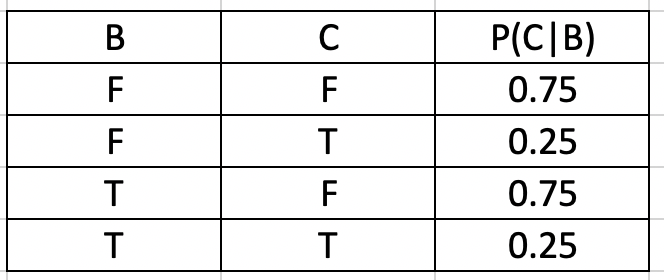
\includegraphics[width=.3\linewidth]{q6p1} 
\end{center}
حال با استفاده از 
\lr{P(B)}
از طریق جدول 
\lr{P(C|B)}
مقدار 
\lr{P(C)}
را به دست می آوریم  :
\begin{center}
				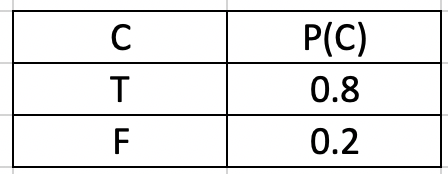
\includegraphics[width=.3\linewidth]{q6p2} 
\end{center}
حال با استفاده از جدول 
\lr{P(C)}
و جدول 
\lr{P(D|C)}
مقادیر 
\lr{P(D)}
را به دست می آوریم  : 
\begin{center}
		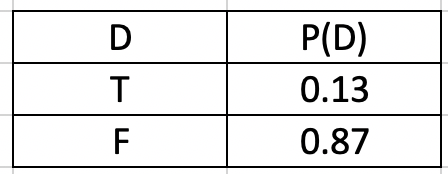
\includegraphics[width=.3\linewidth]{q6p3} 
\end{center}
بنابراین احتمال 
\lr{false}
بودن 
\lr{D}
برابر است با 
\textcolor{red}{0/87}

\end{document}